%%%%%%%%%%%%%%%%%%%%%%%%%%%%%%%%%%%%% BEGIN HEADERS %%%%%%%%%%%%%%%%%%%%%%%%%%%%%%%%%%%%%%%%%%%%%%%%%%%%%
\documentclass[11pt,conference]{IEEEtran}

\usepackage{longtable}
\usepackage{graphicx}
\usepackage[utf8]{inputenc}
\usepackage{fancyhdr}
\usepackage{float}
\usepackage[hidelinks]{hyperref}
\usepackage{listings}
\usepackage{color}
\usepackage{natbib}
\usepackage{caption}

% Your names in the header
\pagestyle{fancy}
\rhead{Enrico Tedeschi, Mike Murphy}
\lhead{INF-3200 Distributed Systems - Assignment 1}
\cfoot{\thepage}

% Used for including code in a stylized manner
\definecolor{codegreen}{rgb}{0,0.6,0}
\definecolor{codegray}{rgb}{0.5,0.5,0.5}
\definecolor{codepurple}{rgb}{0.58,0,0.82}
\definecolor{backcolour}{rgb}{0.95,0.95,0.92}
 

\lstdefinestyle{mystyle}{
    backgroundcolor=\color{backcolour},   
    commentstyle=\color{codegreen},
    keywordstyle=\color{magenta},
    numberstyle=\tiny\color{codegray},
    stringstyle=\color{codepurple},
    basicstyle=\footnotesize,
    breakatwhitespace=false,         
    breaklines=true,                 
    captionpos=b,                    
    keepspaces=true,                 
    numbers=left,                    
    numbersep=5pt,                  
    showspaces=false,                
    showstringspaces=false,
    showtabs=false,                  
    tabsize=2
}

\lstset{style=mystyle}

% The Title
\title{UiT INF-3200 Distributed Systems - Project 1\\Fall 2015}

% Your name and email
\author{Enrico Tedeschi\\ete011@post.uit.no
    \and Mike Murphy\\mmu019@post.uit.no}


%%%%%%%%%%%%%%%%%%%%%%%%%%%%%%%%%%%%% END HEADERS %%%%%%%%%%%%%%%%%%%%%%%%%%%%%%%%%%%%%%%%%%%%%%%%%%%%%

\begin{document}

% Create the title and everything
\maketitle


\section{Introduction}

Our task was to implement a simple distributed key-value store.

The general idea is to have a number of back-end nodes that store data, and a
front-end node that forwards requests into the back-end group. The front-end
should be able to contact any storage node and get the same results.


\subsection{Requirements}

Our data store \ldots

\begin{itemize}
\item must incorporate multiple storage nodes.
\item must work without any node having complete knowledge of the others.
\item must work no matter which storage node the front-end contacts. For
    testing, the front-end should contact random nodes.
\item does not need to support dynamic adding and removal of storage nodes.
\item does not need to persist data between runs.
\end{itemize}


\section{Technical Background}

The basic goal of a distributed database is to coordinate computers so that they
function as if they were a single machine. In a peer-to-peer system with no
designated master node, there must be a deterministic algorithm, shared by all
nodes, that decides which node or nodes should store which values. Each node
must be able to determine whether or not it should be responsible for a given
bit of data, and if not, it must be able to forward the request to the node that
is. With a large number of nodes, it becomes impractical for all nodes to keep a
list of all of the others, so each node will only keep a list of a small number
of neighbors, and the distributed algorithm will have to route requests through
this network of neighbor nodes to the correct location. \cite{p2plookup}

A key-value store lends itself well to this kind of peer-to-peer system, because
the set of possible keys can be viewed as a space to be divided into regions to
be handled by different nodes. The whole system then functions as a distributed
hash table, or DHT. The key questions in designing a DHT system are how the key
space should be divided among nodes, and which nodes should be neighbors and
communicate. \cite{p2plookup}



\section{Design}

In our project, we arranged our key space along one dimension in a ring,
following the lead of Chord\cite{chord}. Regions of the key space are assigned
to each node. Each node is aware of the range of key space that it is
responsible for, and also the next node in the ring (Fig \ref{fig:design}). If a
node receives a request to store or retrieve a key that is not in its range, it
will forward the request to the next node.

Though our design was inspired by Chord, we did not implement Chord's finger
table optimization, for lack of time.

Because all nodes are known ahead of time, with no joining or leaving, we could
divide the key space evenly between each node.

For forwarding requests to successor nodes, we used a simple synchronous
strategy: the node's request-handler thread will block while it contacts the
next node. This was the easiest to implement, but it is wasteful of resources.

\begin{figure}[h!]
  \centering
    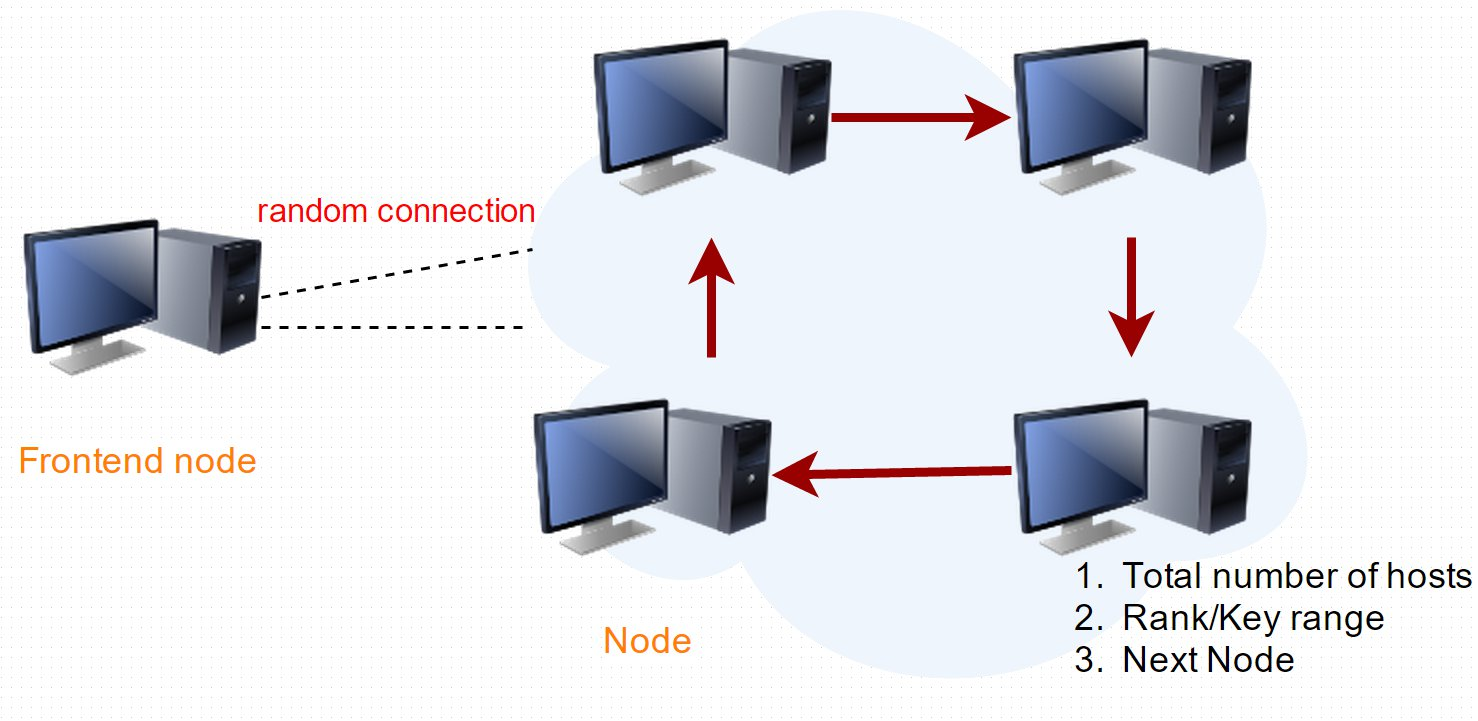
\includegraphics[width=0.5\textwidth]{design}
    \caption{Design of the implemented Network}
    \label{fig:design}
\end{figure}


\section{Implementation}


\subsection{Languages and Code}

Our solution is implemented in a mix of Python and Bash script, Python for the
actual node and front-end programs, and a Bash script to start up and shut down
nodes via SSH.

We started with skeleton code by our teaching assistants, Einar Holsbø Jakobsen
and Magnus Stenhaug, which included the front-end code and the startup/shutdown
shell script. Their front-end also included an automated test routine that
rapidly inserted and retrieved random key-value pairs.

We wrote the actual storage node code, and we also made a few enhancements to
the startup shell script. We modified the startup script to accept its list of
nodes from the command line, rather than a list inside the script itself. We
also added another short script to pick random hosts from the cluster and print
them as a list ready to be copied and pasted into the command line. This made it
easier to randomize which hosts in the cluster we were using, in hopes of
minimizing conflict with other users on the cluster.


\subsection{Network Protocol}

The backend nodes accept and retrieve data through a simple HTTP API. HTTP's PUT
and GET operations are a natural fit for a key-value store, as their semantics
specify storing and retrieving documents (value) at a given URL path (key).
Jakobsen and Stenhaug chose this protocol for their starter front-end node and
we reused it for the storage nodes.


\subsection{Persistence}

The purpose of this exercise was to investigate the challenges of distributed
data storage, not storage itself. Therefore, there was no requirement to
actually persist stored data between runs. So, for simplicity, we did not
implement any kind of data persistence. Data is simply stored in memory and the
store starts empty on each test run.


\subsection{Frontend}

As specified in the requirements, the \textit{Frontend Node} (Fig
\ref{fig:frontend}) contacts a random backend node for each request, and the
backend nodes must cooperate to handle the request. This randomness enforces the
distribution transparency of the data store. The system can store and retrieve
keys as a whole, no matter which individual node is contacted.

\begin{figure}[h!]
  \centering
    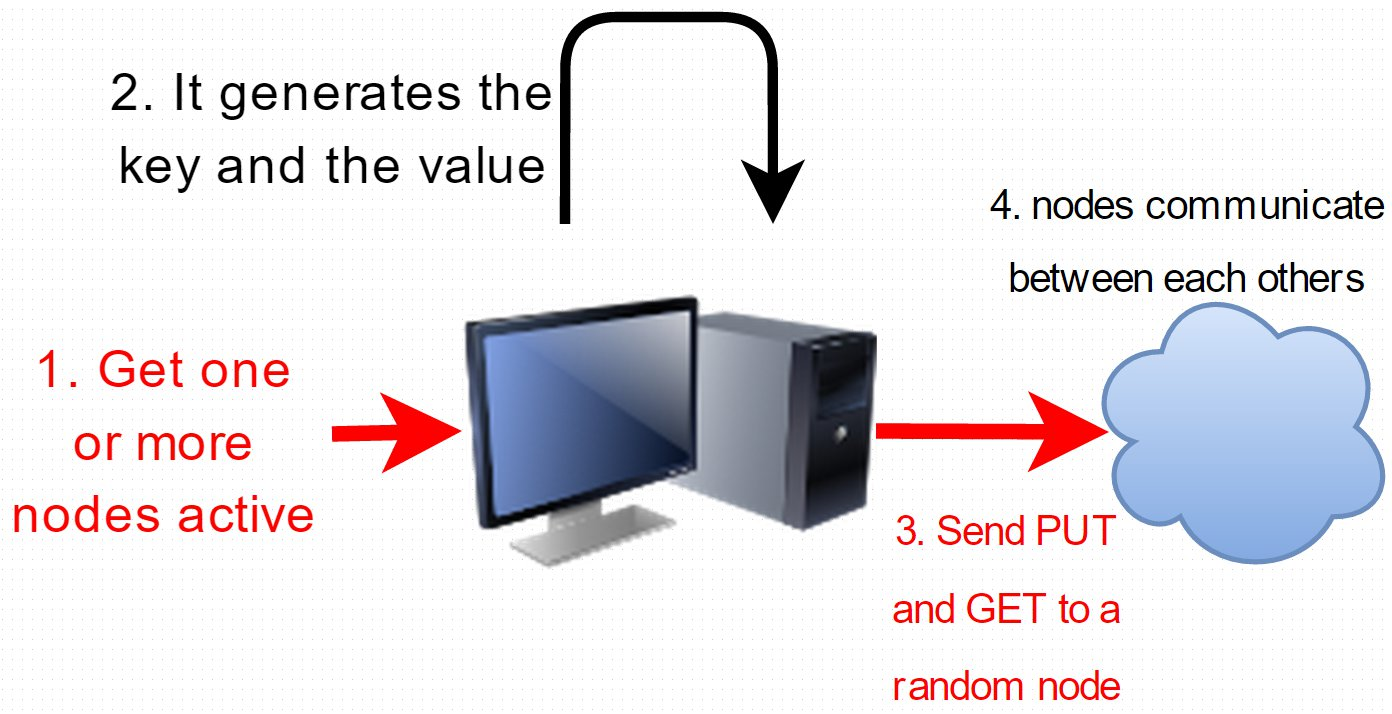
\includegraphics[width=0.5\textwidth]{frontend}
    \caption{Implementation of the Frontend node}
    \label{fig:frontend}
\end{figure}

\subsection{Node}

Each node (Fig \ref{fig:node}) has a simple workflow. It starts running and
waits for a request, which could be GET or PUT from the frontend node or another
backend node. For each request, the node hashes the key into the linear key
space, and checks if it falls within the region assigned to that node. If so,
the node handles the request by storing the value (for PUT) or returning a
previously stored value (for GET). If the key does not fall in the node's
assigned range, it forwards the request to the next node (Fig \ref{fig:putget}).

\begin{figure}[h!]
  \centering
    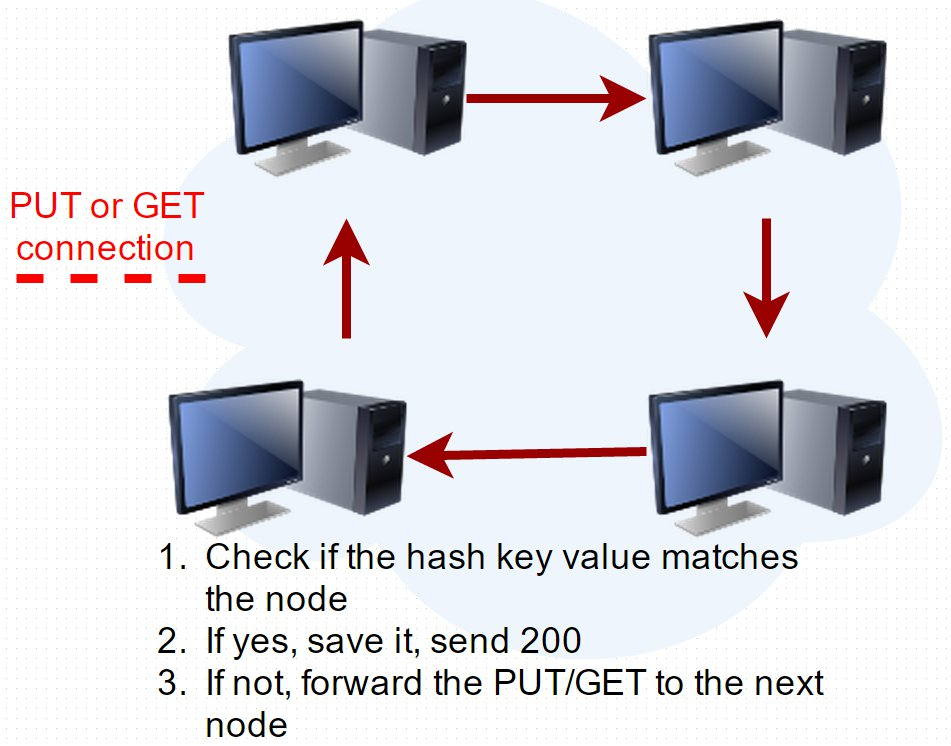
\includegraphics[width=0.5\textwidth]{putget}
    \caption{Implementation of the PUT/GET calls}
    \label{fig:putget}
\end{figure}

The node's logic is split across two classes: \textit{NodeCore} and
\textit{NodeHttpHandler}. \textit{NodeCore} includes the core logic of deciding
when to store a key and when to forward a request to the next node.
\textit{NodeHttpHandler} includes the logic of interpreting HTTP requests and
formatting HTTP responses. This separation of logic makes it possible to verify
the core algorithm with isolated unit tests, without having to set up HTTP
servers.

\begin{figure}[h!]
  \centering
    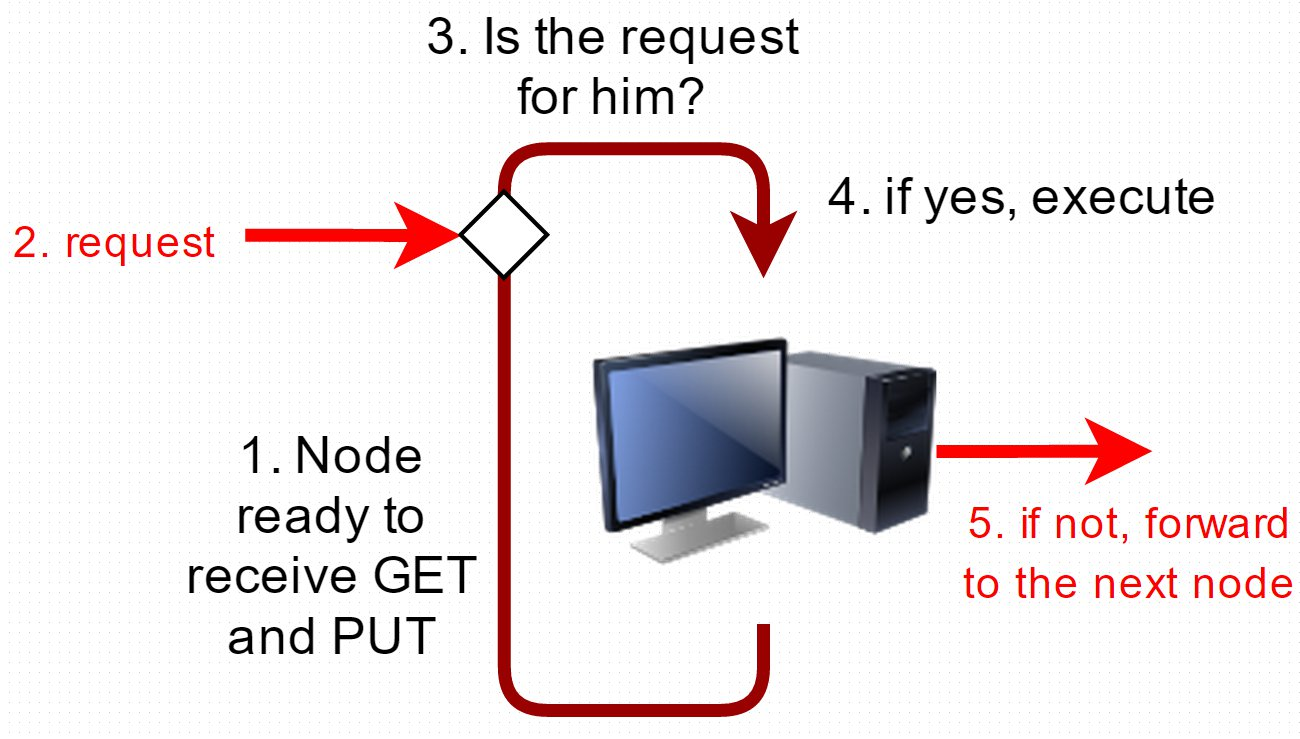
\includegraphics[width=0.5\textwidth]{node}
    \caption{Implementation of Individual Node}
    \label{fig:node}
\end{figure}


For hashing, the node uses the MD5 algorithm to map the string key to a numeric
value, then takes that large integer modulo the number of nodes to get a node
number (Fig \ref{fig:hash_algo}). As a cryptographic algorithm, it is
deterministic and it will evenly distribute the keys. MD5 is also
fast\cite{md5rfc}, so it will not slow down lookups unnecessarily. And though it
no longer considered suitable for security applications\cite{md5badrfc}, it is
not being used for security here. We merely need to decide which node should
store a given key.

\begin{figure}[h!]
\caption{Pseudocode of Core Node Logic}
\begin{lstlisting}
node_responsible = MD5(key) % node_count
if node_responsible == self.rank
then
    save or retrieve value
else
    forward request to next node
\end{lstlisting}
\label{fig:hash_algo}
\end{figure}


\subsection{Environment}

Our code was written to run on the Rocks Cluster distribution\cite{rocks}, and
makes some assumptions about that environment. We rely on the cluster's shared
filesystem for distributing program code to servers. And we rely on easy SSH
access between machines in the cluster to start and shutdown nodes.


\section{Discussion}

Our design decisions favored simplicity over performance. The simple ring
structure was easy to implement, but requests may need to be forwarded along
several nodes in the ring before finding the correct key. The number of hops is
linear with the number of nodes, $O(n)$. Chord's finger-table
optimization\cite{chord} finds nodes in $O(\log_2 n)$ hops. We had hoped to
implement the same strategy in our project but we ran out of time.

The simple synchronous request forwarding strategy is also a potential
bottleneck. It leaves a thread idle on each node involved in each request,
waiting until the right key is found before returning it back through all of the
nodes that were involved. We suspect that, as the number nodes grows or request
frequency increases, this holding of resources will choke the system. The
advantage of this approach is its simplicity. The request and response protocol
is identical between client and front-end, front-end and storage node, and
between storage nodes themselves. The storage nodes also use the same logic to
handle requests whether the request comes from the front-end or another node in
the chain.

Asynchronous message-passing would allow intermediate nodes in a search to free
resources. The first node could block, and then send a message to the next node.
If this message included a return address to the first node, then the other
nodes in the ring could pass it along without leaving connections open or
blocking. Finally, the node that has the key could send the value to original
node. When that original node received its answer, it could unblock and send the
response to the front-end. Such a strategy should be more efficient, but would
require different message formats for requests and answers, and nodes would need
logic to receive answer messages and match them to waiting threads to send
responses. We suspect that the finger tables would give a much larger
performance boost. Not only that, but with $O(\log_2 n)$ searching, only a few
nodes would be involved in each search, and the overhead from waiting
synchronously on just a few nodes might be acceptable.


\section{Evaluation}
For the evaluation node scaling has been considered. The function \textit{storage\_frontend} has been timed sending five hundred requests (GET/PUT) to the nodes network. The evaluation has been done considering the scale on the number of nodes and for each, 10 tests were taken into consideration.
\newline
The number of nodes and the average time of 10 computations is represented in the table in Fig \ref{tab:scaling}.

\begin{figure}[h!]
\centering
% \renewcommand{\figurename}{Fig.}
\caption{Nodes/Time scaling table}
\begin{tabular}[H]{ | l | l | }
\hline
	Nodes & Time \\ \hline
	2 & 5.7923 \\ \hline
	4 & 6.4793 \\ \hline
	6 & 8.1309 \\ \hline
	10 & 13.0746 \\ \hline
	15 & 17.0469 \\ \hline
	20 & 19.3472 \\ \hline
	30 & 29.4729 \\ \hline
	40 & 35.2886 \\ \hline
\end{tabular}
\label{tab:scaling}
\end{figure}

In the Fig \ref{fig:scaling} instead the graphic of this scaling test is characterized.

\begin{figure}[h!]
  \centering
    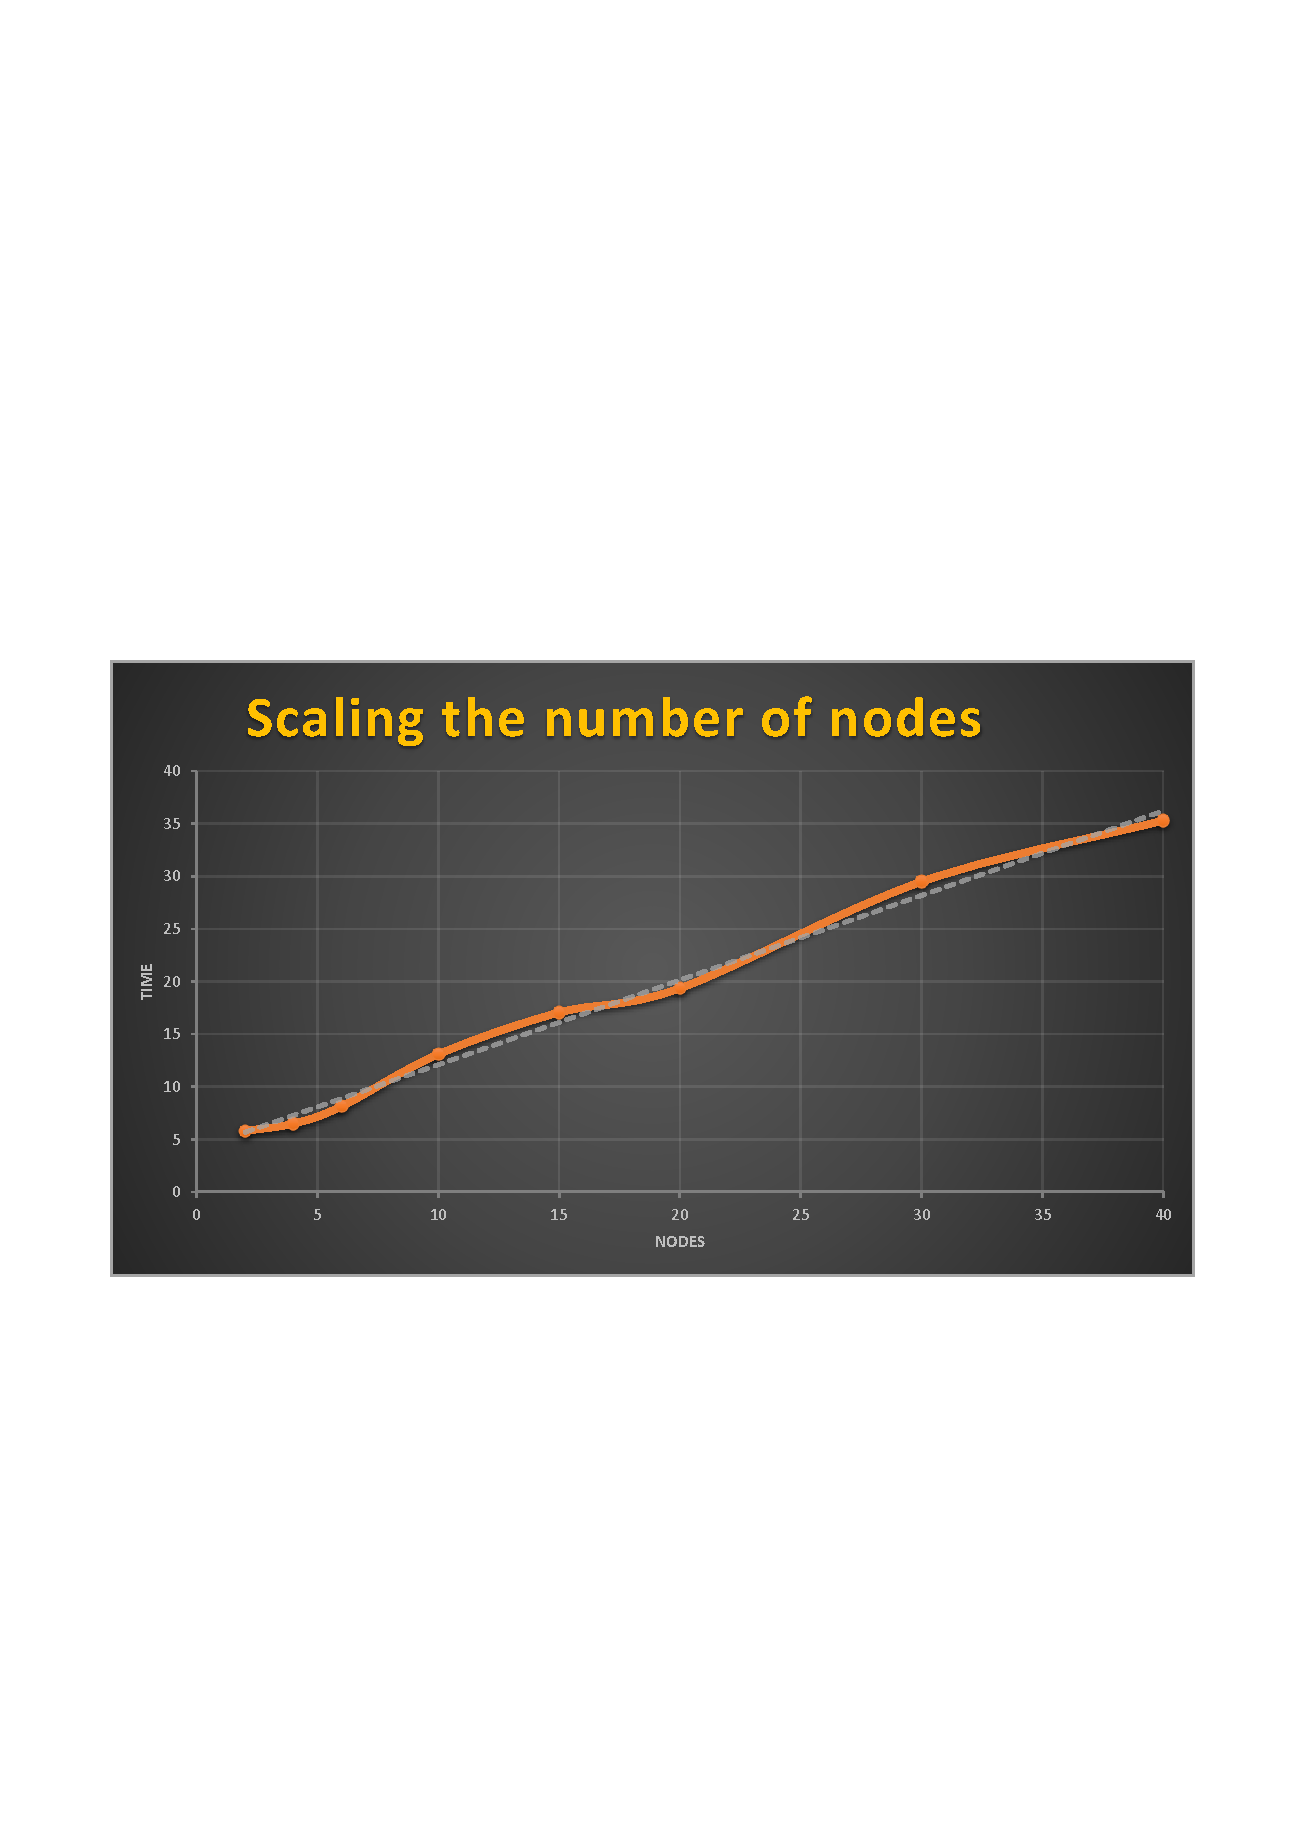
\includegraphics[trim=0cm 9cm 0cm 11cm, width=0.5\textwidth]{scaling}
    \caption{Scaling considering the number of nodes in the network}
    \label{fig:scaling}
\end{figure}


\section{Conclusion}

Our DHT solution, with a simple ring structure, was able to store and retrieve
data correctly, in time that increased linearly with the number of nodes
($O(n)$).


\bibliographystyle{plain}
\bibliography{report}


\end{document}
